% Auto-converted from report/final_report.md

\title{Do Large Language Models Have a Writing Style?\\
\large A Stylometric Comparison of LLM-Generated Texts}
\author{Viola Awor}
\date{}


\maketitle

\begin{abstract}
This report tests whether different large language model (LLM) families exhibit measurable differences in writing style. Using a balanced corpus of 1{,}000 responses from five model families (ChatGPT, Claude, DeepSeek, Gemini, and Mistral) across four genres, 43 stylometric features were extracted and analyzed.

Semantic embedding maps showed little separation by model family (silhouette $=-0.0075$), but stylometric features differed strongly: 41/43 features were significant after FDR correction, and a classifier predicted model family with 78.1\% accuracy (macro F1 = 0.780) under prompt-aware cross-validation.
\end{abstract}

\section{Introduction}
LLMs often produce semantically similar answers to the same prompts, but they may still differ in how they write. This report tests whether model families have measurable stylistic ``fingerprints'' using stylometry: quantitative features capturing sentence structure, punctuation, lexical diversity, and related surface-level patterns.

Five model families (ChatGPT, Claude, DeepSeek, Gemini, and Mistral) generated responses to the same controlled prompt set, producing a balanced corpus of 1{,}000 texts. The analysis compares semantic separability with stylometric separability and evaluates whether stylometric features can predict the generating model family under prompt-aware cross-validation.

\section{Research Question and Methodology}
\subsection{Research question}

\begin{quote}
\textbf{Can stylometric features distinguish texts generated by different large language model families?}
\end{quote}

This question is evaluated through measurable objectives:
\begin{enumerate}
  \item Construct a balanced corpus of LLM-generated texts using controlled prompts.
  \item Extract quantitative stylometric features from each generated output.
  \item Test whether stylometric features differ significantly across model families.
  \item Compare semantic separability with stylometric separability.
  \item Train classifiers to predict the generating model family from stylometric features.
  \item Critically interpret which feature families contribute most to model-family identification.
\end{enumerate}

\subsection{Problem definition}
Let the data set be defined as:
\[
D = \{(x_i, y_i, p_i)\}_{i=1}^{n}
\]
where:
\begin{itemize}
  \item $x_i$ is the generated text;
  \item $y_i$ is the model-family label;
  \item $p_i$ is the prompt identifier;
  \item $n = 1000$ is the number of generated texts.
\end{itemize}

The model-family label belongs to the set:
\[
 y_i \in \{\text{ChatGPT}, \text{Claude}, \text{DeepSeek}, \text{Gemini}, \text{Mistral}\}.
\]

Each text is transformed into a stylometric feature vector:
\[
\phi(x_i) \in \mathbb{R}^{43},
\]
where $\phi(x_i)$ contains 43 stylometric measurements. The supervised classification problem is therefore:
\[
 f: \mathbb{R}^{43} \rightarrow \{1,2,3,4,5\},
\]
where $f$ predicts the model family from the stylometric representation of the text.

\subsection{Dataset design}
The dataset was constructed to reduce confounding effects. Each model family answered the same controlled prompt set. The prompts were distributed across four genres: narrative, descriptive, argumentative, and dialogue. Each generated response was constrained to approximately 180--220 words, with length-control prompts and validation used during data collection.

The final dataset is balanced across both model family and genre.

\begin{table}[H]
\centering
\caption{Dataset summary}
\label{tab:dataset-summary}
\begin{tabular}{lr}
\toprule
Item & Value \\
\midrule
Total generated texts & 1{,}000 \\
Model families & 5 \\
Texts per model family & 200 \\
Genres & 4 \\
Texts per genre & 250 \\
Texts per model family per genre & 50 \\
Stylometric features & 43 \\
Prompt groups & 200 \\
\bottomrule
\end{tabular}
\end{table}

The balance is important because it ensures that classification and statistical testing are not biased by unequal class sizes. Each model contributes the same number of outputs, and each genre is equally represented.

\subsection{Stylometric features}
The project extracts 43 stylometric features from each generated output. These features are grouped into several categories:
\begin{enumerate}
  \item \textbf{Length and sentence structure}
  \begin{itemize}
    \item word count;
    \item character count;
    \item sentence count;
    \item average sentence length;
    \item sentence-length standard deviation;
    \item minimum, maximum, and range of sentence length;
    \item short-sentence ratio;
    \item long-sentence ratio.
  \end{itemize}
  \item \textbf{Punctuation}
  \begin{itemize}
    \item punctuation count;
    \item comma count;
    \item period count;
    \item question-mark count;
    \item exclamation-mark count;
    \item semicolon count;
    \item colon count;
    \item dash count;
    \item quote count;
    \item punctuation rates per 100 words.
  \end{itemize}
  \item \textbf{Casing}
  \begin{itemize}
    \item uppercase word count;
    \item titlecase word count;
    \item uppercase character ratio.
  \end{itemize}
  \item \textbf{Lexical diversity}
  \begin{itemize}
    \item type-token ratio;
    \item hapax legomena ratio;
    \item repeated word ratio;
    \item Yule's K;
    \item Simpson diversity;
    \item Honore's R;
    \item moving-average type-token ratio.
  \end{itemize}
  \item \textbf{Discourse and marker features}
  \begin{itemize}
    \item function-word count;
    \item function-word ratio;
    \item transition-marker count and ratio;
    \item hedging-marker count and ratio;
    \item AI-style marker count and ratio.
  \end{itemize}
  \item \textbf{Readability}
  \begin{itemize}
    \item Flesch reading ease;
    \item Gunning Fog index.
  \end{itemize}
\end{enumerate}

These features are designed to capture not only what the models write about, but how they write.

\subsection{Semantic mapping}
To compare stylometric separability with semantic separability, sentence embeddings were generated for the texts. Dimensionality reduction was applied using PCA and t-SNE. Clustering quality was measured with cosine silhouette scores for three labels: model family, genre, and theme.

The silhouette score measures how close points are to other points in the same group compared with points in other groups. For a point $i$, the silhouette value is:
\[
 s(i) = \frac{b(i)-a(i)}{\max(a(i), b(i))},
\]
where $a(i)$ is the average distance from point $i$ to other points in the same group, and $b(i)$ is the average distance from point $i$ to the nearest different group.

Values close to 1 indicate strong clustering, values close to 0 indicate overlap, and negative values indicate that points may be closer to another group than to their assigned group.

\subsection{Statistical testing}
For each stylometric feature, a Kruskal--Wallis test was used to test whether feature distributions differ across model families. This non-parametric test is appropriate because stylometric features may not be normally distributed.

The hypotheses for each feature are:
\[
H_0: F_{\text{ChatGPT}} = F_{\text{Claude}} = F_{\text{DeepSeek}} = F_{\text{Gemini}} = F_{\text{Mistral}},
\]
\[
H_1: \text{At least one model-family distribution differs.}
\]

Because 43 features are tested, $p$-values were corrected using the Benjamini--Hochberg false discovery rate procedure. Effect size was measured using epsilon-squared:
\[
\epsilon^2 = \frac{H-k+1}{n-k},
\]
where $H$ is the Kruskal--Wallis statistic, $k$ is the number of groups, and $n$ is the total number of observations.

Pairwise Mann--Whitney U post-hoc tests were then used on the strongest features to identify which model pairs drive the omnibus differences.

\subsection{Classification methodology}
Two classifiers were evaluated: Logistic Regression and Random Forest.

The classifiers were trained on four feature sets: (1) all 43 stylometric features; (2) content-oriented features; (3) structure/format features; (4) features without structure/format features.

A prompt-aware GroupKFold cross-validation strategy was used. The grouping variable was \texttt{prompt\_id}, meaning the same prompt never appears in both training and testing folds. This is critical because all models answer the same prompt set. Without grouping by prompt, the classifier could learn prompt-specific topic patterns instead of model-specific writing style.

Classification performance was evaluated using accuracy, macro precision, macro recall, macro F1, and weighted F1. Accuracy is defined as:
\[
\text{Accuracy} = \frac{\text{Number of correct predictions}}{\text{Total number of predictions}}.
\]

For each class $c$, precision and recall are:
\[
\text{Precision}_c = \frac{TP_c}{TP_c + FP_c},
\qquad
\text{Recall}_c = \frac{TP_c}{TP_c + FN_c}.
\]

The class-specific F1-score is:
\[
F1_c = 2 \cdot \frac{\text{Precision}_c \cdot \text{Recall}_c}{\text{Precision}_c + \text{Recall}_c}.
\]

Macro F1 is the unweighted average across the $K=5$ model families:
\[
\text{MacroF1} = \frac{1}{K}\sum_{c=1}^{K}F1_c.
\]

Because there are five balanced classes, the random baseline is:
\[
\frac{1}{5} = 0.20.
\]

\section{Experimental Results}
\subsection{Dataset verification}
The final dataset contains 1,000 generated texts and 43 stylometric features. Each of the five model families contributes exactly 200 texts, and each genre contributes 250 texts. Within each model-family and genre combination, there are 50 texts.

This confirms that the dataset is balanced and appropriate for model-family comparison.

\subsection{Semantic mapping results}
Sentence embeddings were used to test whether generated texts cluster naturally by model family, genre, or theme.

\begin{table}[ht]
\centering
\caption{Semantic silhouette scores}
\label{tab:semantic-silhouette}
\begin{tabular}{lr}
\toprule
Label & Cosine silhouette score \\
\midrule
Theme & 0.0685 \\
Genre & 0.0361 \\
Model family & -0.0075 \\
\bottomrule
\end{tabular}
\end{table}

\begin{figure}[H]
\centering
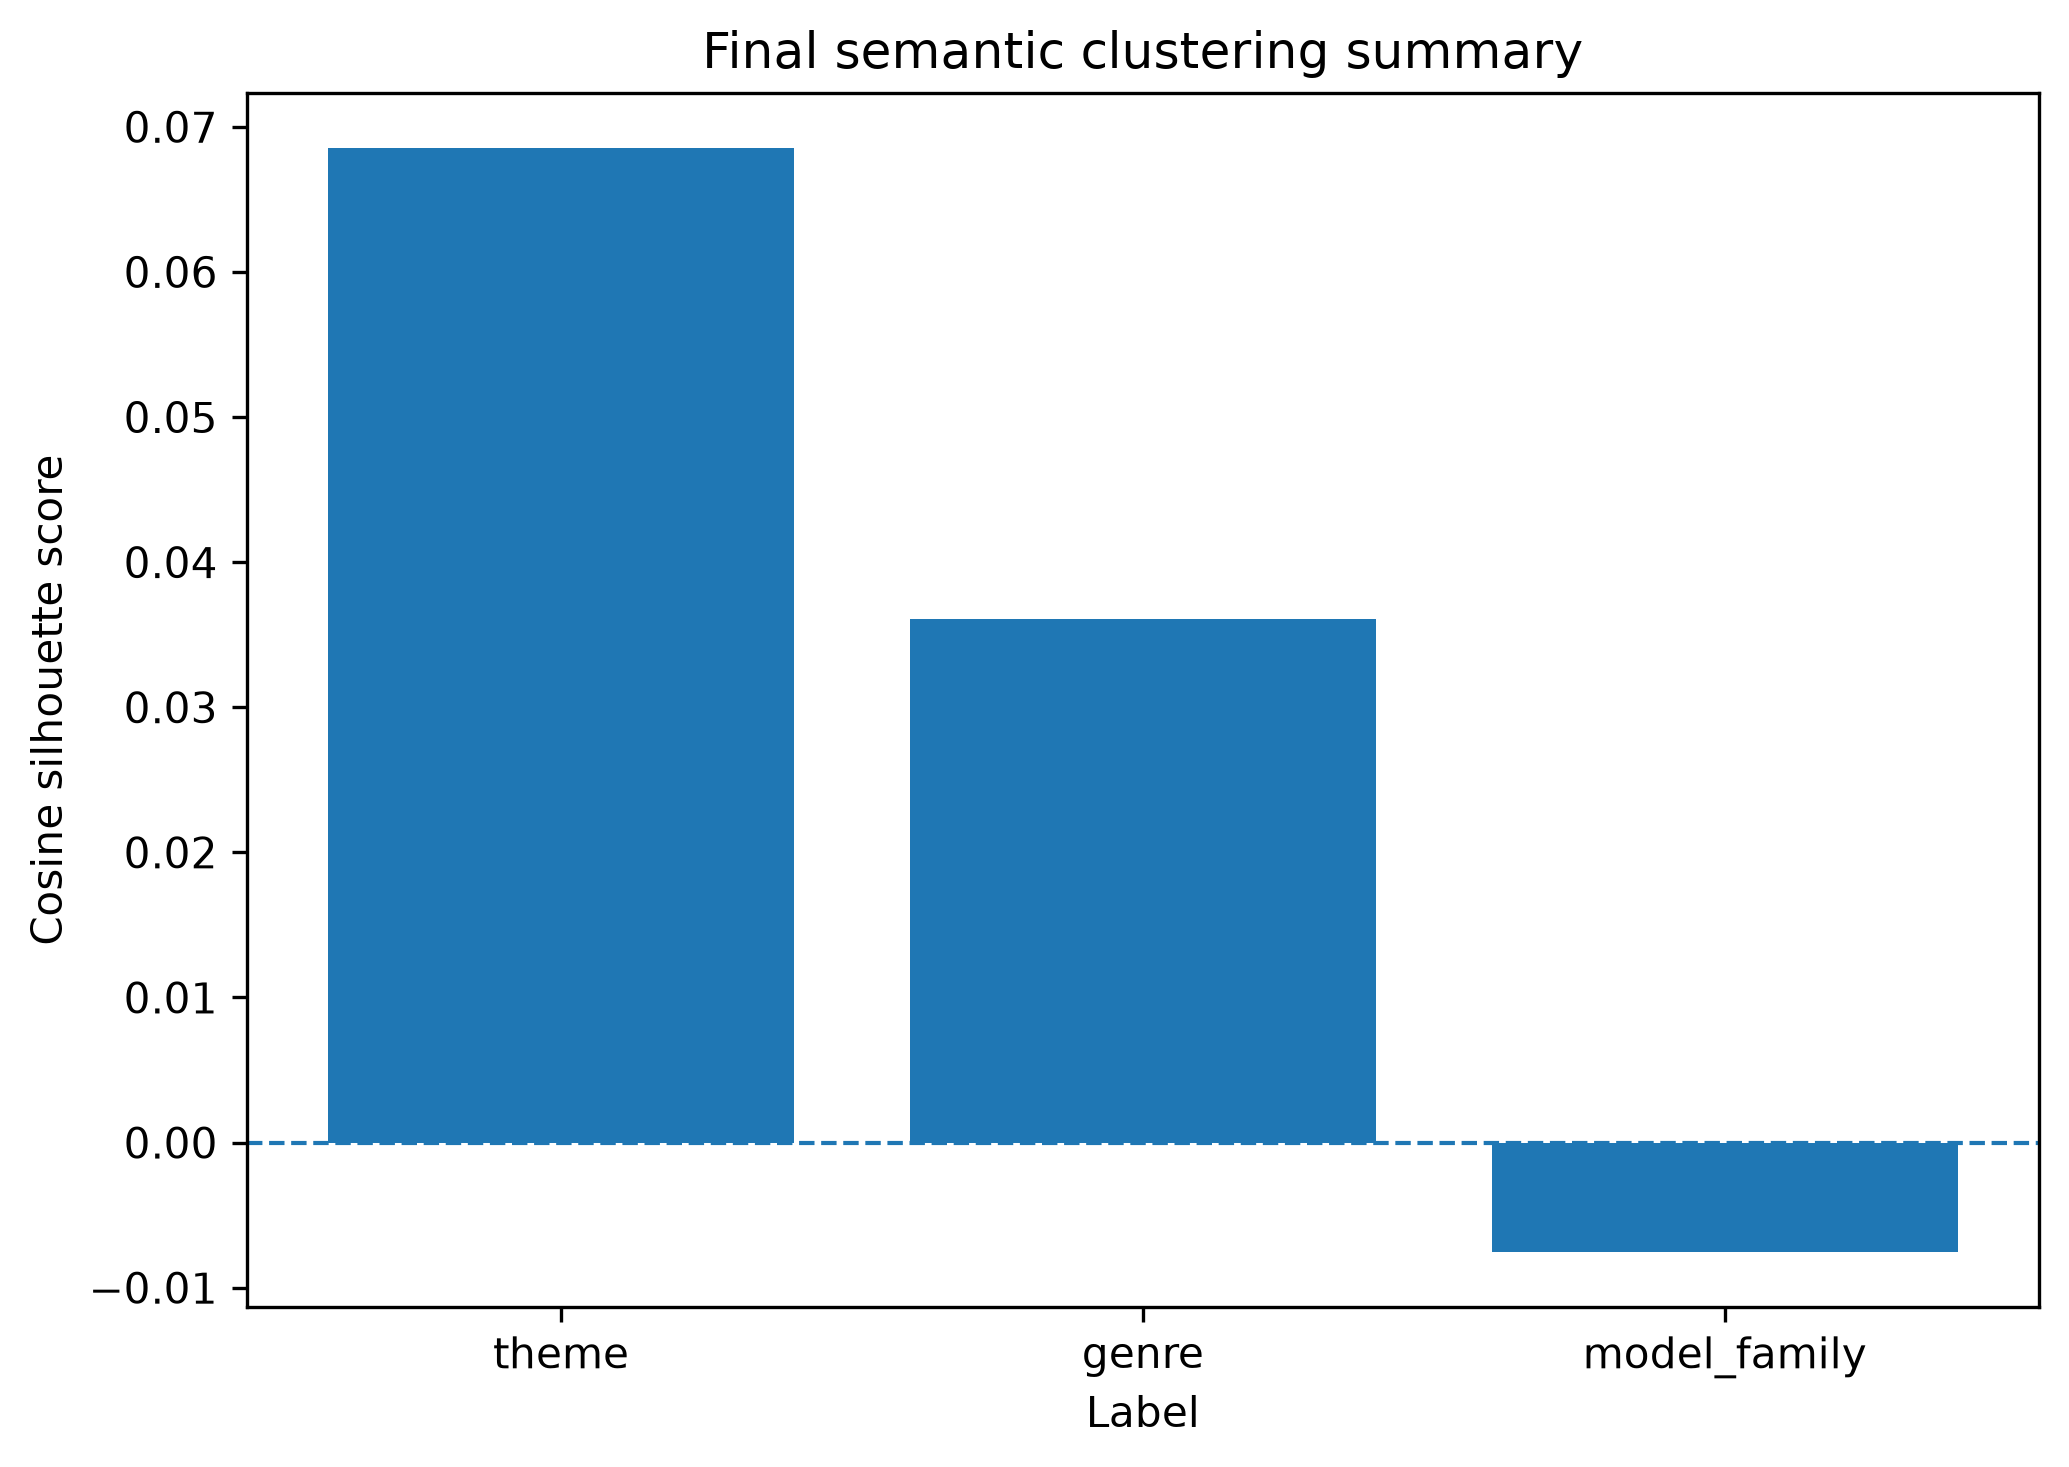
\includegraphics{outputs/figures/final_semantic_silhouette_summary.png}
\caption{Semantic silhouette summary.}
\label{fig:semantic-silhouette-summary}
\end{figure}

The semantic results show weak clustering overall. Theme has the highest silhouette score, but the value is still low. Genre has a weaker positive value. Model family has a slightly negative score.

This means that sentence embeddings do not naturally separate texts according to the generating LLM family. The models are producing semantically similar responses to the same prompts. This is an important result because it shows that model identity is not strongly visible in general semantic space.

Therefore, if model-family identity is detectable, it is more likely to appear in stylometric features than in broad semantic similarity.

\subsection{Statistical testing results}
The Kruskal--Wallis tests show strong differences across model families.

\begin{table}[ht]
\centering
\caption{Statistical-test summary}
\label{tab:stat-test-summary}
\begin{tabular}{lr}
\toprule
Item & Value \\
\midrule
Total stylometric features tested & 43 \\
Significant after FDR correction & 41 \\
Not significant after FDR correction & 2 \\
Share significant & 0.9535 \\
Large effect features & 22 \\
Medium effect features & 7 \\
Small effect features & 11 \\
Negligible effect features & 3 \\
\bottomrule
\end{tabular}
\end{table}

\begin{figure}[H]
\centering
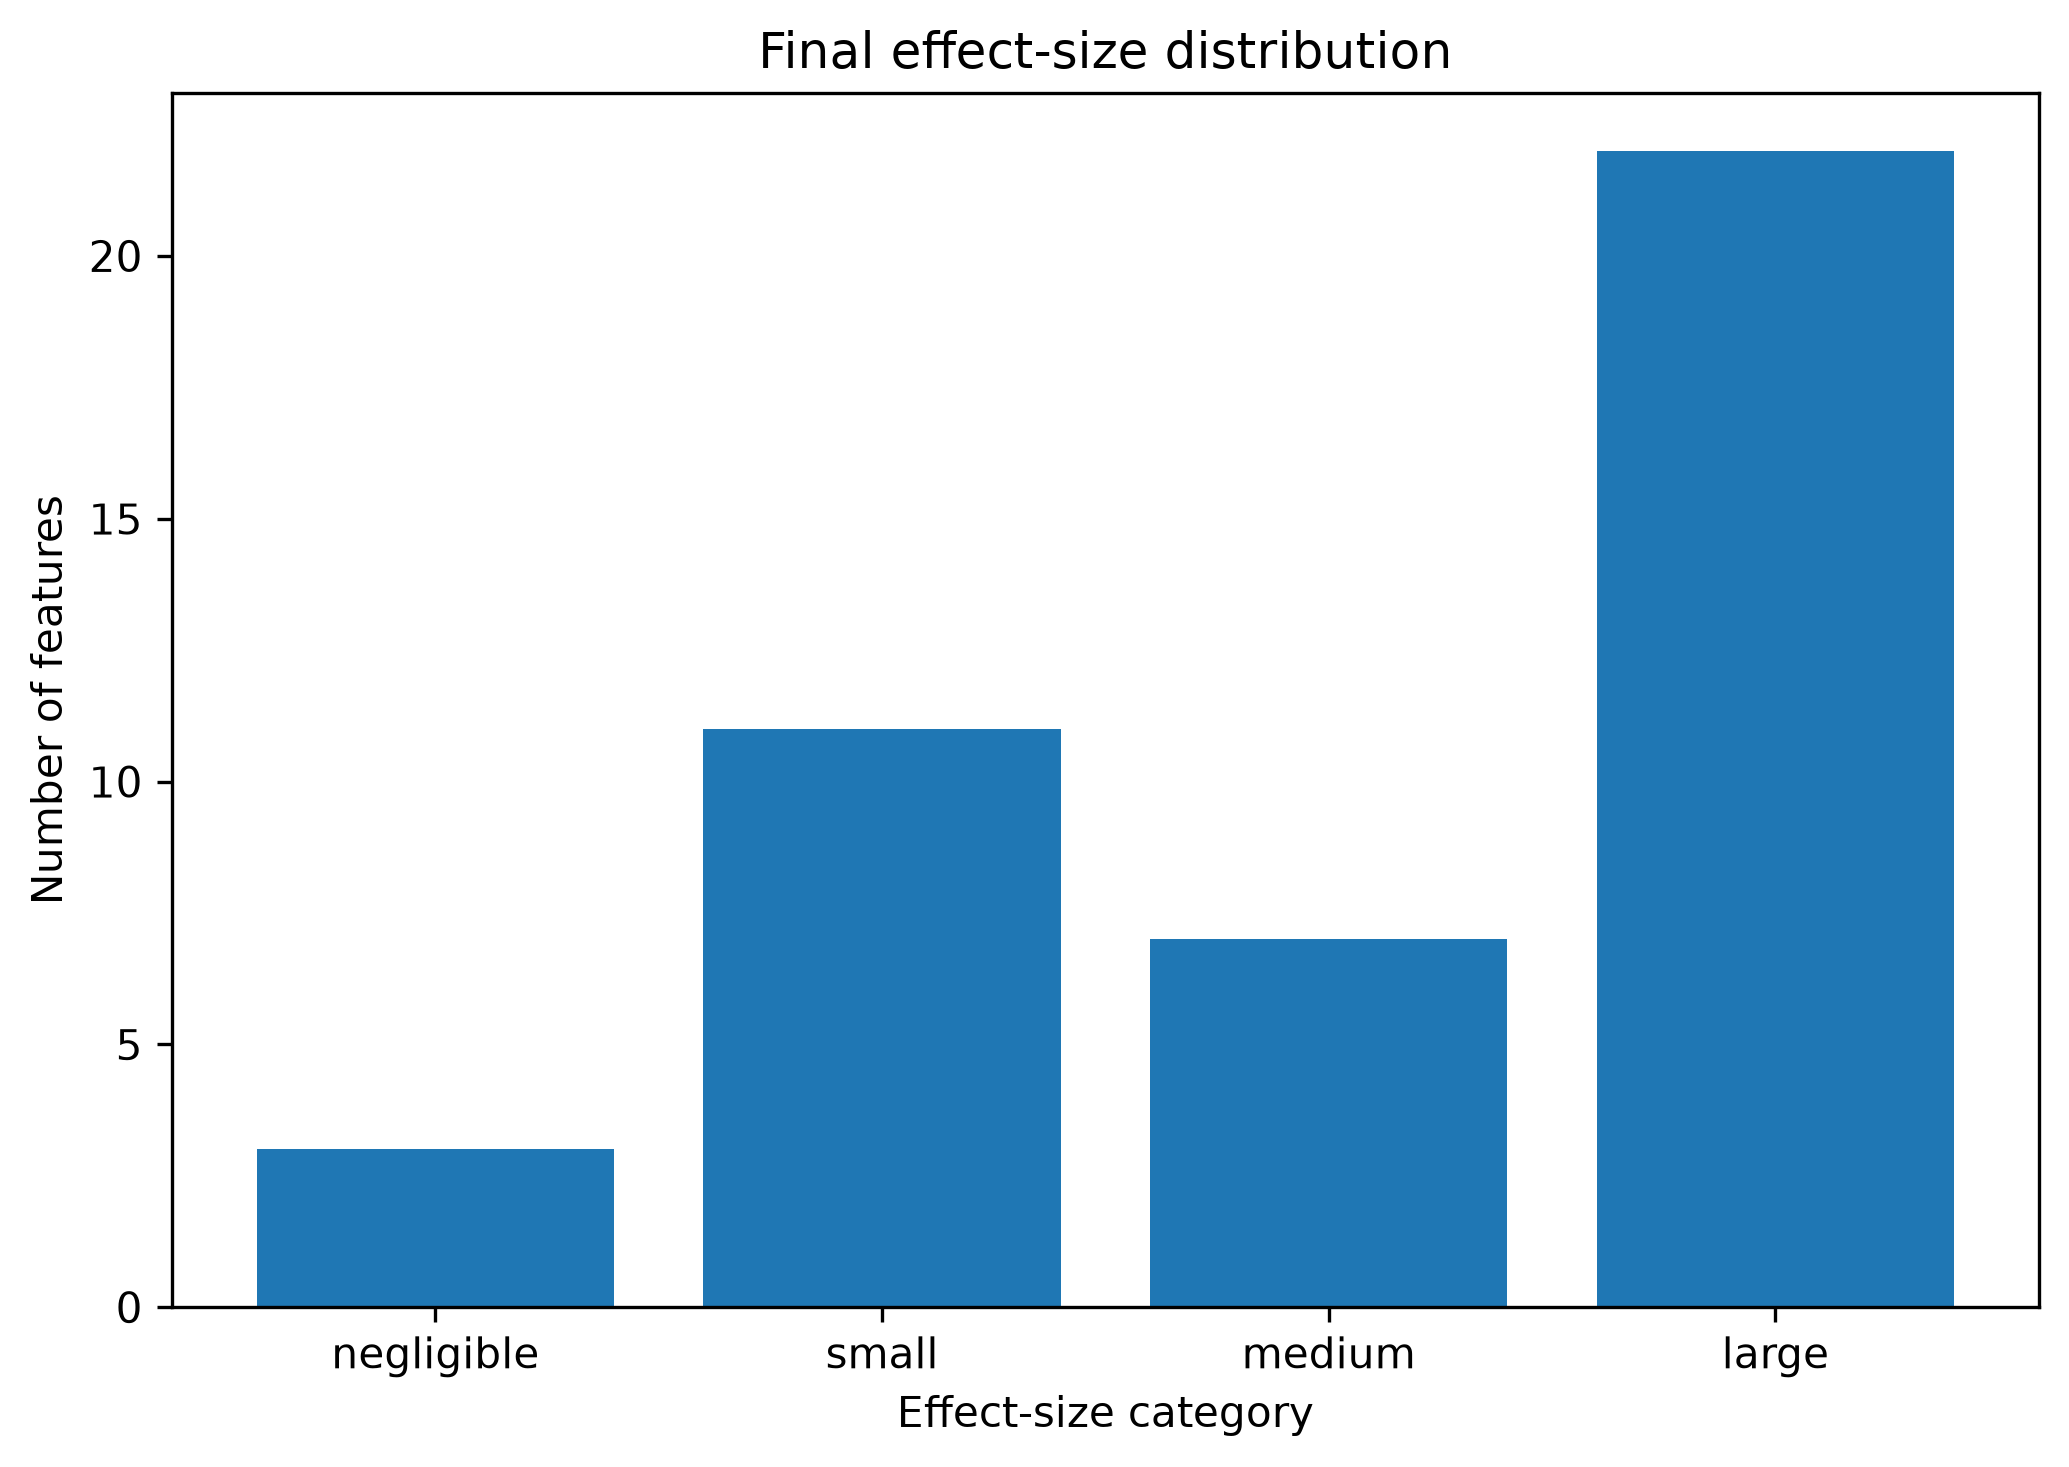
\includegraphics{outputs/figures/final_effect_size_distribution.png}
\caption{Effect-size distribution.}
\label{fig:effect-size-distribution}
\end{figure}

Out of 43 features, 41 are significant after FDR correction. This means that the majority of stylometric features differ across ChatGPT, Claude, DeepSeek, Gemini, and Mistral.

The effect sizes strengthen the interpretation. Twenty-two features have large effects, and seven have medium effects. Therefore, the differences are not only statistically detectable; many are practically meaningful.

The strongest model-family differences occur in features related to sentence length, punctuation, word count, function-word usage, average word length, character density, lexical diversity, readability, and AI-style marker usage.

Several important model-specific tendencies emerge from the top statistical features:
\begin{itemize}
  \item \textbf{DeepSeek} tends to have higher word count, longer sentence maxima, higher long-sentence ratio, greater sentence-length variability, and higher function-word count.
  \item \textbf{Gemini} shows especially high comma count and comma density.
  \item \textbf{Claude} has higher average word length, character count, type-token ratio, and period density.
  \item \textbf{ChatGPT} shows a higher function-word ratio.
\end{itemize}

These differences suggest that model families are not merely separated by one isolated feature. Instead, their writing-style differences are distributed across several stylometric dimensions.

\subsection{Genre-specific robustness}
The statistical tests were also repeated within each genre.

\begin{table}[ht]
\centering
\caption{Genre-specific robustness}
\label{tab:genre-robustness}
\begin{tabular}{lr}
\toprule
Genre & Significant features \\
\midrule
Argumentative & 40 / 43 \\
Narrative & 39 / 43 \\
Dialogue & 38 / 43 \\
Descriptive & 37 / 43 \\
\bottomrule
\end{tabular}
\end{table}

The model-family signal persists across all four genres. This means the stylometric differences are not caused by only one genre or prompt type. Even when the analysis is restricted to argumentative, narrative, dialogue, or descriptive texts, most features remain significantly different across model families.

This result supports the robustness of the methodology.

\subsection{Post-hoc testing results}
The omnibus Kruskal--Wallis tests show that at least one model family differs for each feature, but they do not identify which model pairs differ. Therefore, pairwise Mann--Whitney U post-hoc tests were conducted on the strongest features.

\begin{table}[ht]
\centering
\caption{Post-hoc summary}
\label{tab:posthoc-summary}
\begin{tabular}{lr}
\toprule
Item & Value \\
\midrule
Total pairwise post-hoc tests & 100 \\
Significant after FDR correction & 86 \\
Share significant & 0.86 \\
\bottomrule
\end{tabular}
\end{table}

The post-hoc results show that the global differences are driven by concrete model-to-model contrasts. Examples include DeepSeek producing longer outputs than ChatGPT and Mistral, Gemini using more commas than Claude, and Claude having higher average word length than DeepSeek.

This makes the statistical evidence more interpretable. The model-family differences are not vague; they correspond to specific stylistic contrasts between particular models.

\subsection{Classification results}
The classification experiment tests whether stylometric features can predict the generating model family. The dataset contains five balanced model classes, so the random baseline is 20\%.

\begin{table}[ht]
\centering
\caption{Classification performance summary}
\label{tab:classification-summary}
\begin{tabular}{llrr}
\toprule
Classifier & Feature set & Accuracy & Macro F1 \\
\midrule
Logistic Regression & All stylometric features & 0.781 & 0.780 \\
Random Forest & All stylometric features & 0.779 & 0.776 \\
Random Forest & Structure/format features & 0.745 & 0.742 \\
Logistic Regression & Structure/format features & 0.722 & 0.720 \\
Logistic Regression & Content-oriented features & 0.602 & 0.599 \\
Random Forest & Content-oriented features & 0.571 & 0.562 \\
\bottomrule
\end{tabular}
\end{table}

\begin{figure}[H]
\centering
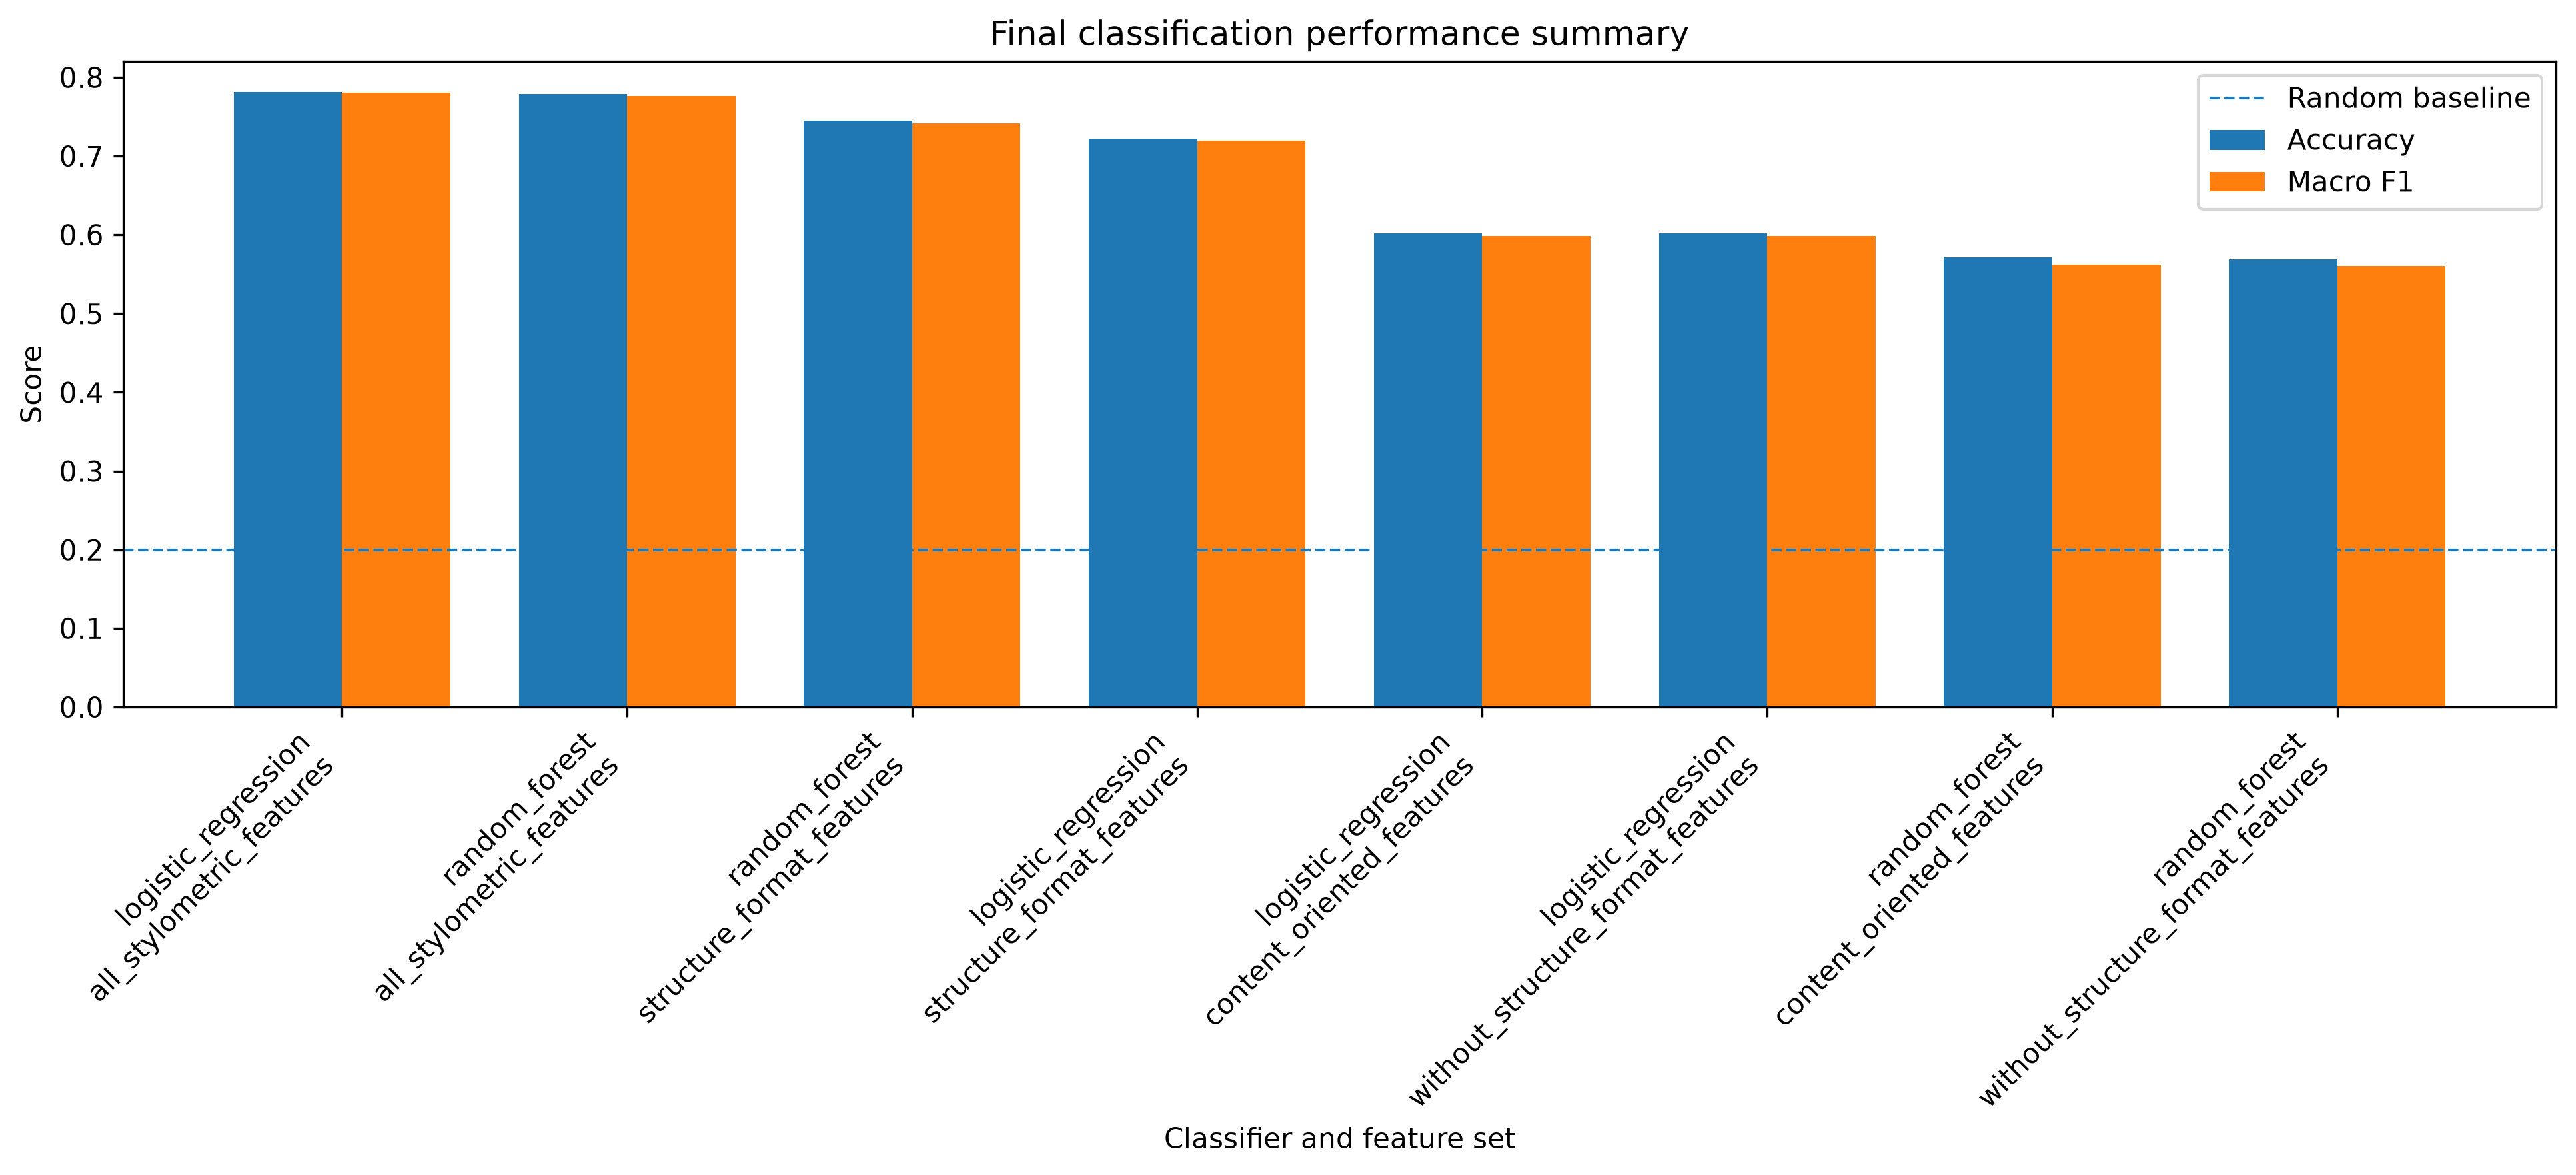
\includegraphics{outputs/figures/final_classification_performance_summary.png}
\caption{Classification performance summary.}
\label{fig:classification-performance-summary}
\end{figure}

The best classifier is Logistic Regression using all 43 stylometric features. It achieves 78.1\% accuracy and 0.780 macro F1. Random Forest using all stylometric features performs almost identically, reaching 77.9\% accuracy and 0.776 macro F1.

These results are far above the 20\% random baseline. This provides strong predictive evidence that stylometric features contain model-family information.

The feature-set comparison is also informative. Structure/format features alone achieve up to 74.5\% accuracy, while content-oriented features reach approximately 60.2\% accuracy. This suggests that model identity is especially visible in formal writing patterns such as sentence length, punctuation, word count, character density, and casing.

The use of prompt-aware GroupKFold cross-validation makes this result stronger. Since the same prompt IDs are not shared across training and testing folds, the classifier is less likely to exploit prompt memorization or topic leakage. The result therefore supports the interpretation that the classifier is learning model-family writing-style signals.

\subsection{Feature importance}
Random Forest feature importance was used to inspect which stylometric features contribute most to prediction.

\begin{figure}[H]
\centering
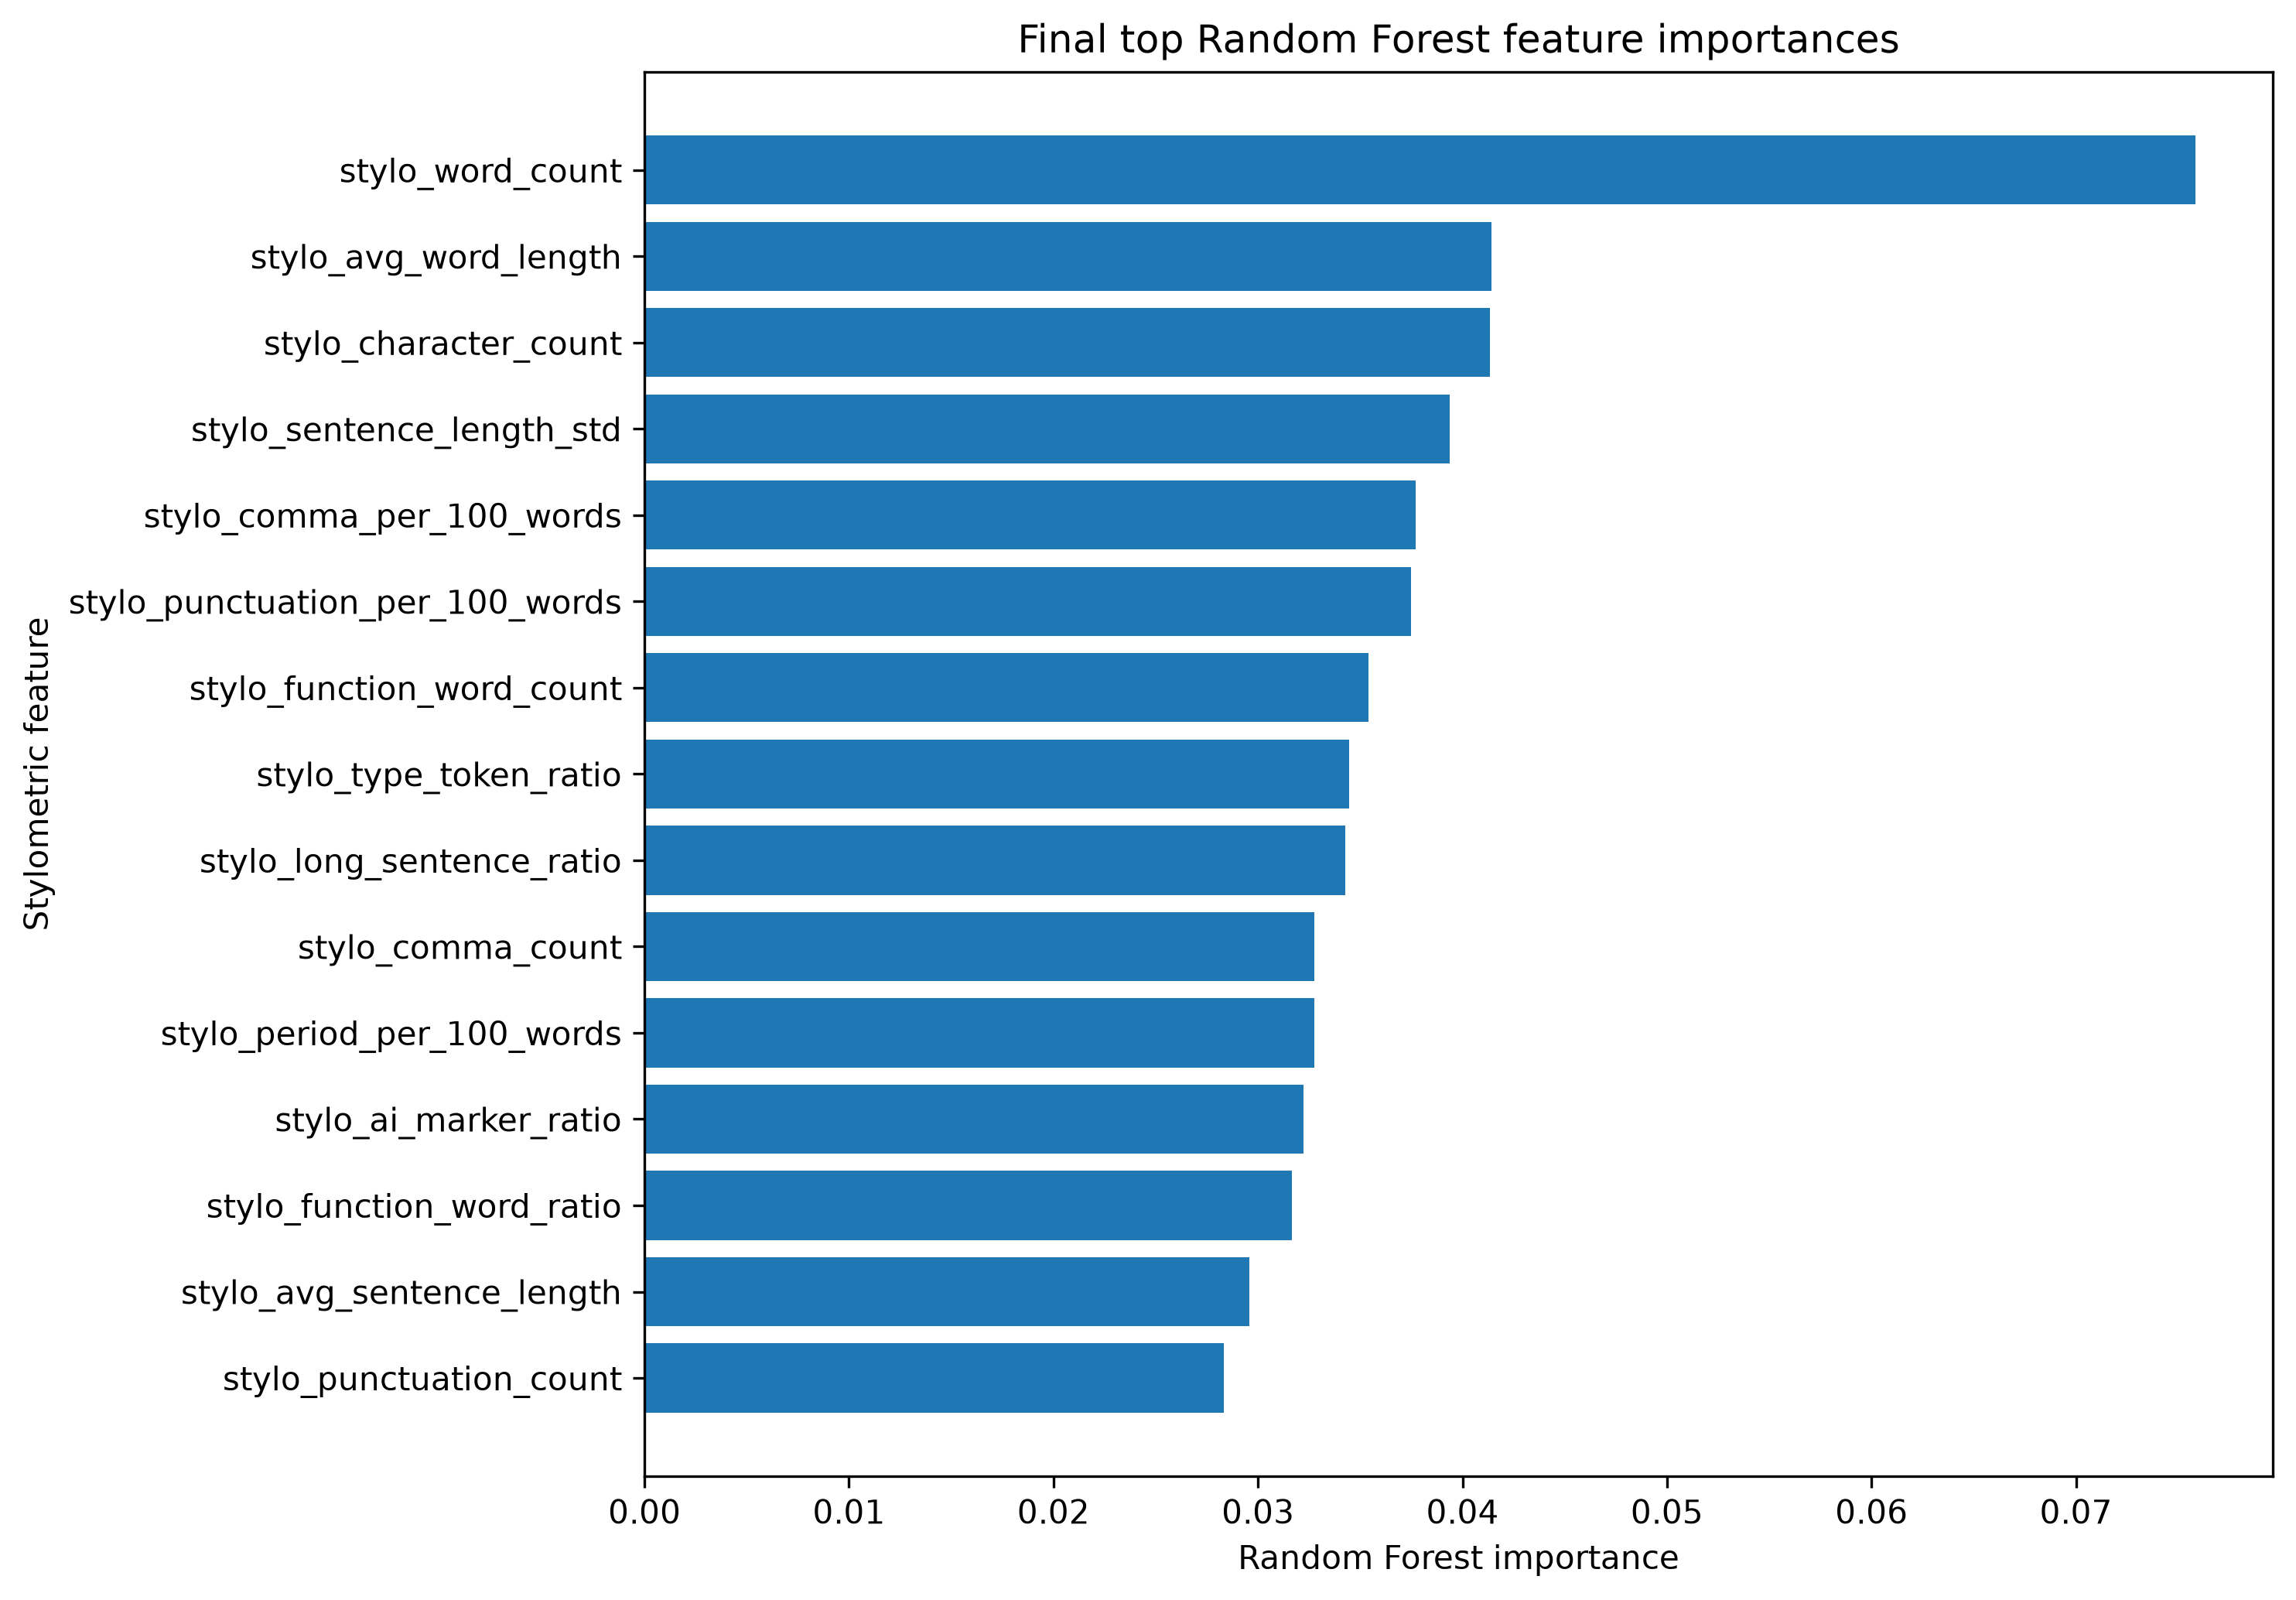
\includegraphics{outputs/figures/final_top_feature_importance.png}
\caption{Top feature importance.}
\label{fig:top-feature-importance}
\end{figure}

The most important features are concentrated in structural, punctuation, lexical, and marker-based dimensions. This matches the statistical results, where sentence length, comma usage, word count, function-word usage, average word length, and lexical diversity were among the strongest model-family differences.

The feature-family importance summary shows that model identity is distributed across multiple categories of writing style.

\begin{figure}[H]
\centering
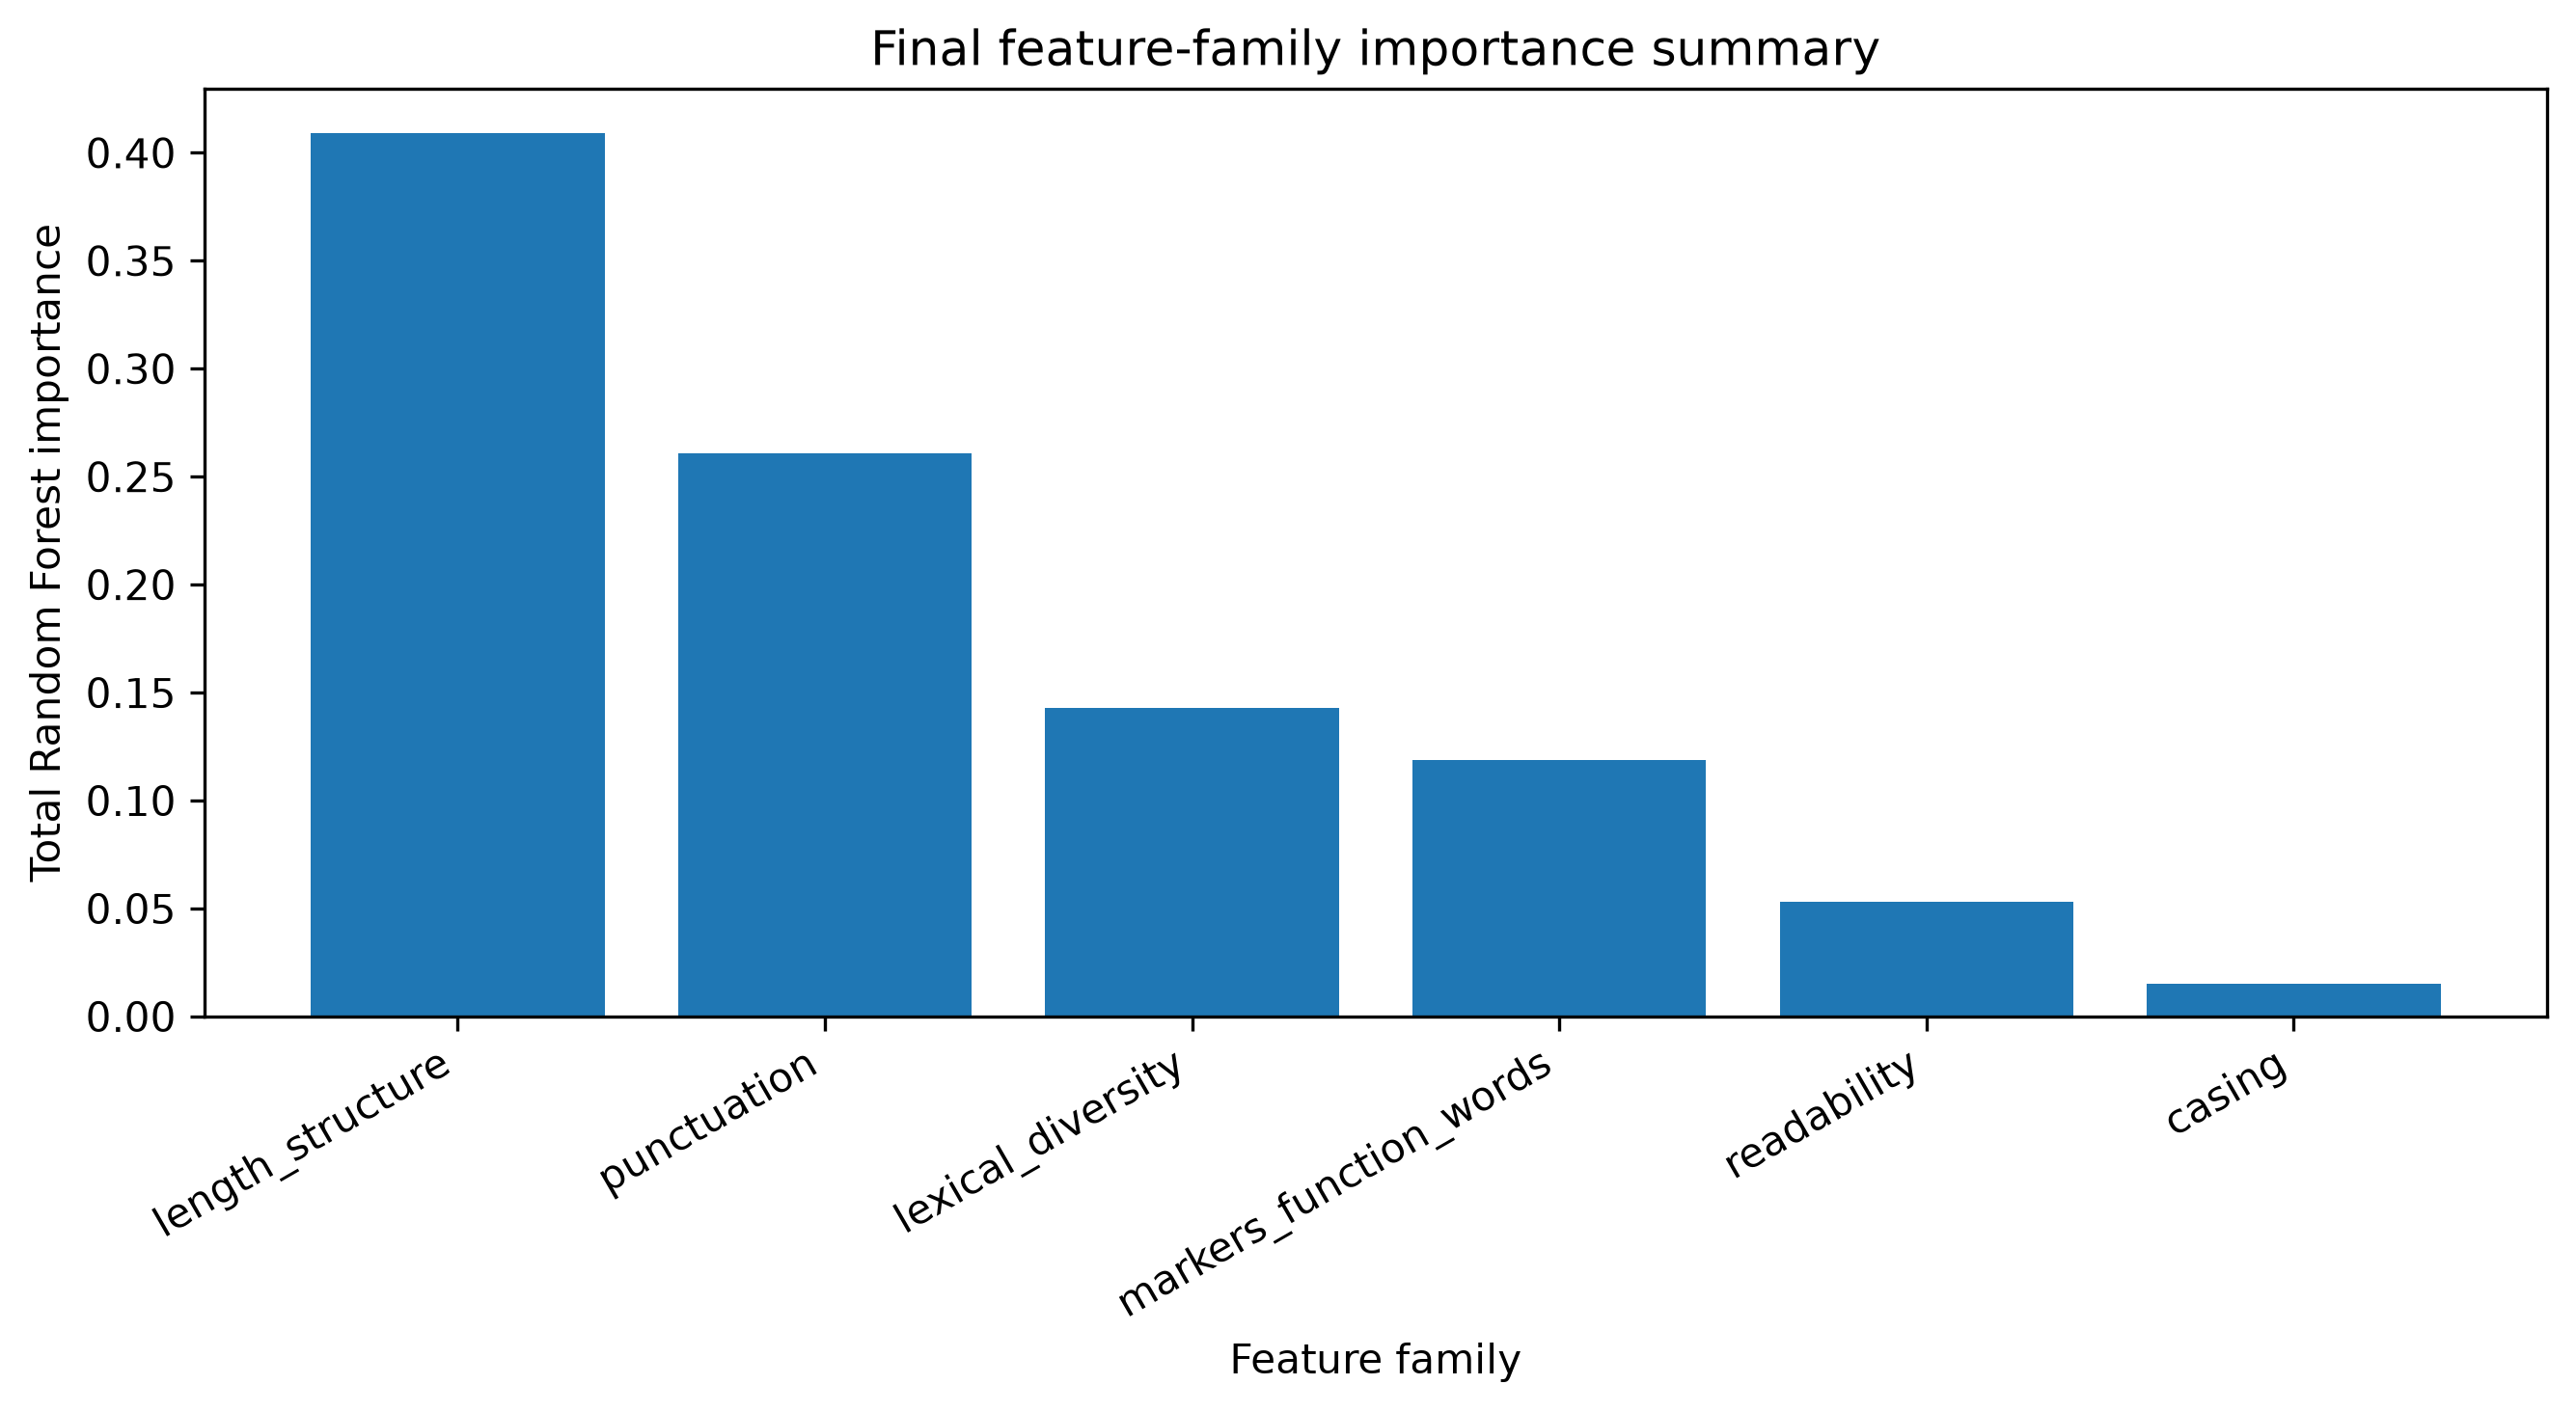
\includegraphics{outputs/figures/final_feature_family_importance.png}
\caption{Feature-family importance.}
\label{fig:feature-family-importance}
\end{figure}

The main conclusion from feature importance is that model-family identity is not encoded in one isolated variable. Instead, it appears as a distributed stylistic profile across sentence structure, punctuation, lexical diversity, readability, and marker-based features.

\subsection{Streamlit dashboard}
A Streamlit dashboard was implemented as an interactive presentation layer for the project. The dashboard loads the saved outputs from the analysis pipeline and presents dataset summary, stylometric feature exploration, semantic maps, statistical-test results, classification performance, feature importance, and the final conclusion.

The app does not replace the report or the notebooks. Instead, it supports reproducibility and interpretability by allowing users to inspect the main results interactively.

\section{Concluding Remarks}
This project investigated whether LLM-generated texts contain measurable model-specific writing styles. The final answer is yes: stylometric features can distinguish texts generated by different LLM families far above chance.

The semantic analysis showed that model-family identity is not strongly visible in general sentence-embedding space. The model-family silhouette score was slightly negative, while theme had the strongest but still weak semantic signal. This suggests that the models produce semantically similar responses to the same prompts.

In contrast, stylometric analysis revealed strong model-family differences. Forty-one out of 43 stylometric features were significant after FDR correction, and 22 features had large effects. These differences persisted across genres and were supported by post-hoc pairwise testing.

The classification results provided the strongest predictive evidence. Logistic Regression using all stylometric features achieved 78.1\% accuracy and 0.780 macro F1 under prompt-aware cross-validation. Since the random baseline is 20\%, the classifier performs almost four times better than chance. Structure/format features alone achieved up to 74.5\% accuracy, showing that formal writing patterns are especially informative.

The critical interpretation is that this project does not prove that model identity can always be perfectly detected. Instead, it shows that under a controlled experimental design, different LLM families leave measurable writing-style fingerprints. These fingerprints are visible in sentence structure, punctuation, word count, character density, lexical diversity, function-word usage, readability, and marker-based features.

\subsection{Limitations}
Key limitations are: (i) the study uses a single controlled prompt set and a fixed set of model versions/settings, so stylistic patterns may shift across tasks or after model updates; (ii) the dataset is limited to 1{,}000 English texts across four genres and five model families; and (iii) the feature set (43 stylometric variables) captures surface style and may miss deeper syntactic or discourse-level signals.

\subsection{Future work}
Future work could (i) broaden coverage (more models/versions, tasks, and languages), (ii) test robustness under model updates and paraphrasing, and (iii) expand beyond surface stylometry with richer syntactic and discourse features.

Overall, the project demonstrates that stylometry is a useful methodology for analyzing LLM-generated writing. Even when generated texts are semantically similar, they can still differ in measurable writing-style patterns. This supports the central conclusion that large language models do not only generate content; they also generate style.

\section{Reproducibility}
The project is organized as a reproducible Python repository. The main logic is separated into scripts and modules, while notebooks are used for demonstration, interpretation, and visualization.

The repository contains data loading and preprocessing modules, model-output generation scripts, stylometric feature extraction code, semantic mapping code, statistical testing code, classification modeling code, a Streamlit dashboard, and saved outputs, tables, and figures.

The main scripts can be run from the project root:
\begin{verbatim}
python scripts/generate_outputs.py
python scripts/preprocess_outputs.py
python scripts/extract_features.py
python scripts/feature_summary.py
python scripts/create_semantic_maps.py
python scripts/run_statistical_tests.py
python scripts/run_classification_modeling.py
streamlit run app/streamlit_dashboard.py
\end{verbatim}

\section{References and tools}
Tools used include Python (pandas, NumPy, scikit-learn, SciPy, statsmodels, matplotlib), sentence-transformers, and Streamlit.

% Bibliography will print even if there are currently no citations.
\printbibliography


